\documentclass[11pt,letterpaper]{article}
\usepackage{fontspec}
\usepackage[spanish,es-noshorthands,es-tabla]{babel}
\usepackage{plantilla/unab_propuesta}

% Los datos compartidos se generan desde datos.md al ejecutar compilar.py.
\input{.build/datos.tex}
\hypersetup{pdftitle={\TituloTrabajo},pdfauthor={\Docente}}

\begin{document}
\pagestyle{empty}

% =========================================================================
% PÁGINA 1: ENCABEZADO, OBJETIVOS, INDICACIONES GENERALES, FASES Y CRONOGRAMA
% =========================================================================
\encabezadoguia

\noindent{\fontsize{11}{13}\selectfont\textbf{OBJETIVOS DE LA ACTIVIDAD}}\par
\vspace{0.3em}

\noindent{\fontsize{10.5}{12.5}\selectfont\textbf{Objetivo General}}\par
\vspace{0.2em}
{\fontsize{10}{12.5}\selectfont Diseñar e implementar un prototipo funcional de circuito digital integrado con microcontroladores que responda a una problemática ambiental real, aplicando simplificación booleana, compuertas lógicas, integrados combinacionales y maquetado físico.\par}

\vspace{0.4em}
\noindent{\fontsize{10.5}{12.5}\selectfont\textbf{Objetivos Específicos}}\par
\vspace{0.2em}
\begin{itemize}[leftmargin=1.5em,label=\flecha,itemsep=0.2em,topsep=0.1em]
  \item Identificar y delimitar una problemática ambiental concreta, definiendo la población beneficiaria y el impacto del sistema propuesto.
  \item Modelar el comportamiento lógico del sistema mediante tablas de verdad, ecuaciones booleanas y la inclusión explícita de módulos multiplexores (MUX) o demultiplexores (DEMUX).
  \item Simular el circuito completo en la plataforma A+ (o Tinkercad/Logisim) previo al ensamble físico.
  \item Construir una maqueta funcional utilizando Arduino, circuitos integrados digitales (TTL/CMOS) y técnicas de ensamblaje físico (cableado, soldadura en placa perforada o PCB).
  \item Redactar un informe técnico formal bajo los estándares de publicación IEEE.
\end{itemize}

\vspace{0.5em}
\noindent{\fontsize{11}{13}\selectfont\textbf{INDICACIONES GENERALES Y DINÁMICA DE TRABAJO}}\par
\vspace{0.3em}

\begin{itemize}[leftmargin=1.5em,label=\cuadrado,itemsep=0.35em,topsep=0.1em]
  \item \textbf{Conformación de Equipos:} Los estudiantes trabajarán estrictamente en grupos de 4 integrantes.
  \item \textbf{Eje Temático (Medio Ambiente):} El proyecto debe resolver o monitorear un problema ambiental (gestión de residuos, ahorro energético, calidad del aire/agua, automatización de riego sustentable, detección de incendios, control de huella de carbono, entre otros).
  \item \textbf{Validación Obligatoria de Propuesta:} Antes de iniciar cualquier compra o ensamble, el grupo debe someter su propuesta formal al docente. \textbf{Ningún proyecto podrá desarrollarse sin la validación y firma de aprobación previa del catedrático.}
  \item \textbf{Requisitos Técnicos Mínimos del Hardware:}
  \begin{itemize}[leftmargin=1.5em,label=$\circ$,itemsep=0.25em,topsep=0.15em]
    \item \textbf{Circuitería Lógica Pura:} Debe incluir al menos una etapa basada en lógica combinacional discreta (compuertas lógicas integradas, tablas de verdad optimizadas por Mapas de Karnaugh).
    \item \textbf{Módulos MUX / DEMUX:} Integración funcional de al menos un integrado multiplexor o demultiplexor (ej. 74LS151, 74LS138, 74HC4051).
    \item \textbf{Microcontrolador (Arduino):} Procesamiento de señales de sensores ambientales y control de actuadores o despliegue de datos.
    \item \textbf{Maquetado y Soldadura:} La entrega final requiere una maqueta física a escala donde la circuitería esté soldada de forma limpia en placas perforadas/PCB y cableada adecuadamente.
  \end{itemize}
\end{itemize}

\vspace{0.5em}
\noindent{\fontsize{11}{13}\selectfont\textbf{FASES Y CRONOGRAMA DE ENTREGAS}}\par

\clearpage

% =========================================================================
% PÁGINA 2: FASE 1 - NOMBRE DEL PROYECTO, INTEGRANTES, PROBLEMÁTICA Y JUSTIFICACIÓN
% =========================================================================

\noindent{\fontsize{11}{13}\selectfont\textbf{Fase 1: Ficha de Propuesta de Proyecto (Entrega para Validación)}}\par
\vspace{0.25em}
\noindent{\fontsize{10.5}{12.5}\selectfont El equipo entregará un documento de un máximo de dos páginas que contenga:}\par

\vspace{0.4em}
\begin{itemize}[leftmargin=1.5em,itemsep=0.2em,topsep=0.1em]
  \item \textbf{Nombre del proyecto y miembros del equipo.}
\end{itemize}

\vspace{0.25em}
\noindent
\begin{tabularx}{\linewidth}{|>{\raggedright\arraybackslash}p{2.8cm}|X|>{\raggedright\arraybackslash}p{1.7cm}|>{\raggedright\arraybackslash}p{3.2cm}|}
  \hline
  \textbf{Nombre del Proyecto:} & \multicolumn{3}{>{\raggedright\arraybackslash}X|}{\TituloTrabajo} \\
  \hline
  \multicolumn{4}{|l|}{\textbf{Integrantes del Equipo (4 estudiantes)}} \\
  \hline
  \textbf{Estudiante (Líder):} & \IntegrantesLiderNombre & \textbf{Carnet:} & \IntegrantesLiderCodigo \\
  \hline
  \textbf{Estudiante:} & \IntegrantesDosNombre & \textbf{Carnet:} & \IntegrantesDosCodigo \\
  \hline
  \textbf{Estudiante:} & \IntegrantesTresNombre & \textbf{Carnet:} & \IntegrantesTresCodigo \\
  \hline
  \textbf{Estudiante:} & \IntegrantesCuatroNombre & \textbf{Carnet:} & \IntegrantesCuatroCodigo \\
  \hline
\end{tabularx}

\vspace{0.8em}
\begin{itemize}[leftmargin=1.5em,itemsep=0.2em,topsep=0.1em]
  \item \textbf{Problemática ambiental identificada y justificación.}
  \item \textbf{Población objetivo y beneficiarios directos.}
\end{itemize}

\vspace{0.25em}
\noindent
\begin{tabularx}{\linewidth}{|X|}
  \hline
  \textbf{Problemática Ambiental Identificada:}\par\vspace{0.3em}
  {\fontsize{9.5}{12}\selectfont En San Miguel, El Salvador, las lluvias torrenciales y ondas tropicales provocan incrementos críticos del caudal en la cuenca del Río Grande de San Miguel y severas acumulaciones pluviales en sectores urbanos como la colonia Palo Blanco, debido a deficiencias del drenaje e inundaciones repentinas. La dependencia de inspecciones visuales manuales limita el tiempo de respuesta comunitario, evidenciando la necesidad de investigar un sistema digital continuo de monitoreo del nivel de agua con comunicación de advertencias tempranas.\par}
  \vspace{0.4em}
  \\
  \hline
  \textbf{Justificación:}\par\vspace{0.3em}
  {\fontsize{9.5}{12}\selectfont El desarrollo de un prototipo digital de bajo costo permite detectar de forma automatizada niveles críticos de agua combinando sensores ultrasónicos y de flotador. La integración de lógica combinacional pura mediante compuertas físicas (AND, OR, NOT) asegura una validación robusta y prefiltrado de umbrales en hardware antes del procesamiento, mientras que la tecnología LoRa garantiza la transmisión inalámbrica de estados hacia una estación receptora comunitaria sin depender de infraestructura Wi-Fi o telefonía celular, decodificando las alertas mediante un demultiplexor físico (DEMUX).\par}
  \vspace{0.4em}
  \\
  \hline
  \textbf{Población Objetivo y Beneficiarios Directos:}\par\vspace{0.4em}
  \textbf{Población Objetivo:} {\fontsize{9.5}{12}\selectfont Habitantes y familias de la colonia Palo Blanco (San Miguel Centro, distrito con 74,650 hogares según el Censo de Población y Vivienda 2024 de la ONEC/BCR), específicamente aquellos domicilios ubicados en sectores vulnerables a inundaciones repentinas y saturación de drenajes pluviales.\par}\vspace{0.3em}
  \textbf{Beneficiarios Directos:} {\fontsize{9.5}{12}\selectfont Cantidad de beneficiarios directos pendiente de delimitación y verificación (familias residentes en el área proyectada de cobertura del nodo receptor, con un núcleo inicial de aproximadamente 15 a 30 familias en calle y senda Los Laureles que registran antecedentes documentados de anegamientos e inundaciones recurrentes según informes de Protección Civil y prensa local).\par}
  \vspace{0.4em}
  \\
  \hline
\end{tabularx}

\clearpage

% =========================================================================
% PÁGINA 3: DIAGRAMA DE BLOQUES Y PRESUPUESTO ESTIMADO
% =========================================================================

\begin{itemize}[leftmargin=1.5em,itemsep=0.2em,topsep=0.1em]
  \item \textbf{Diagrama de bloques preliminar del sistema (Sensores, Lógica Combinacional / MUX / DEMUX, Arduino, Actuadores).}
\end{itemize}

\vspace{0.2em}
\begin{center}
  \vspace*{-0.2em}
  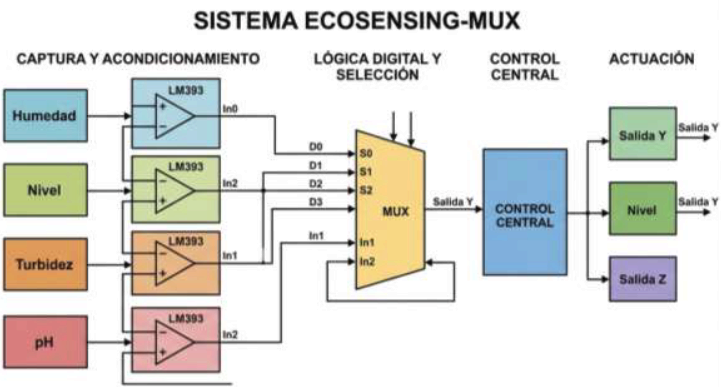
\includegraphics[width=0.88\linewidth,height=7.4cm,keepaspectratio]{assets/img/circuito.png}
\end{center}

\vspace{-0.2em}
\begin{itemize}[leftmargin=1.5em,itemsep=0.1em,topsep=0.1em]
  \item \textbf{Presupuesto estimado y lista de materiales a utilizar.}
\end{itemize}

\vspace{0.1em}
\vspace{0.15em}
{\small\renewcommand{\arraystretch}{0.92}%
\begin{tabularx}{\linewidth}{|>{\centering\arraybackslash}p{0.75cm}|>{\raggedright\arraybackslash}X|>{\raggedright\arraybackslash}X|>{\centering\arraybackslash}p{1.75cm}|>{\centering\arraybackslash}p{1.75cm}|}
  \hline
  \textbf{Cant.} & \textbf{Descripción del Material / Componente} & \textbf{Aplicación en el Proyecto} & \textbf{\shortstack{Costo Unitario\\(\$)}} & \textbf{\shortstack{Costo Total\\(\$)}} \\
  \hline
  1 & Arduino Uno & Procesamiento y lectura de sensores (Estación A) & \$5.10 & \$5.10 \\
  \hline
  2 & Módulos ESP32 NodeMCU & Control y gestión de enlace LoRa (Estación A y B) & \$4.37 & \$8.74 \\
  \hline
  2 & Módulos LoRa RFM95 / SX1276 & Enlace inalámbrico de advertencia a larga distancia & \$7.25 & \$14.50 \\
  \hline
  2 & Antenas omnidireccionales LoRa 6 dBi & Radiación y recepción de señal RF & \$15.63 & \$31.26 \\
  \hline
  1 & Sensor ultrasónico impermeable JSN-SR04T & Medición continua de distancia a la lámina de agua & \$2.12 & \$2.12 \\
  \hline
  3 & Interruptores de nivel tipo flotador & Detección discreta de umbrales físicos (F1, F2, F3) & \$1.29 & \$3.87 \\
  \hline
  1 & CI 74HC08 (AND) / CI 74HC32 (OR) & Lógica combinacional física de validación & \$1.09 & \$1.09 \\
  \hline
  1 & CI 74HC04 (NOT) / CI 74HC238 (DEMUX) & Inversión de señales y decodificación de alertas & \$2.02 & \$2.02 \\
  \hline
  4 & LEDs indicadores / Mini buzzer BGD08 & Señalización visual y acústica en Estación B & \$1.80 & \$1.80 \\
  \hline
  4 & Baquelas perforadas soldables (mod. 400/405) & Base física y montaje soldado de circuitería & \$2.49 & \$9.96 \\
  \hline
  1 & Soldadura SOL60-020 y Alambre estañado & Ensamblado permanente y conexionado físico & \$5.99 & \$5.99 \\
  \hline
  --- & Materiales de Maqueta (Estructura/Cauce) & Simulación física de cauce y entorno comunitario & \$12.00 & \$12.00 \\
  \hline
  --- & Accesorios USB y Regulación 3.3V & Adaptación de niveles lógicos y potencia & \$12.14 & \$12.14 \\
  \hline
  \multicolumn{4}{|r|}{\textbf{TOTAL ESTIMADO}} & \textbf{\$110.59} \\
  \hline
\end{tabularx}%
}

\clearpage

% =========================================================================
% PÁGINA 4: FIRMAS DE VALIDACIÓN, FASE 2 Y DETALLE DE SECCIONES (PARTE 1)
% =========================================================================

\begin{itemize}[leftmargin=1.5em,itemsep=0.2em,topsep=0.1em]
  \item \textbf{Firmas de conformidad y validación}
\end{itemize}

\vspace{0.25em}
\noindent
\begin{tabularx}{\linewidth}{|X|}
  \hline
  \vspace{0.15em}
  \textbf{Firma del Líder del Equipo}\par\vspace{0.2em}
  Fecha de entrega: \rule{1.2cm}{0.4pt} / \rule{1.2cm}{0.4pt} / \rule{1.8cm}{0.4pt}\par\vspace{0.5em}
  \textbf{RESERVADO PARA EL DOCENTE DE LA ASIGNATURA:}\par\vspace{0.2em}
  \begin{itemize}[leftmargin=1.5em,itemsep=0.15em,topsep=0.1em]
    \item \textbf{Dictamen:} [~~] APROBADO \quad [~~] RECHAZADO \quad [~~] REVISAR Y REENVIAR
    \item \textbf{Observaciones / Modificaciones sugeridas:}
  \end{itemize}
  \vspace{1.1cm}
  \textbf{Firma y Sello del Catedrático}\par\vspace{0.2em}
  Fecha de validación: \rule{1.2cm}{0.4pt} / \rule{1.2cm}{0.4pt} / \rule{1.8cm}{0.4pt}\par\vspace{0.3em}
  \\
  \hline
\end{tabularx}

\vspace{0.8em}
\noindent{\fontsize{10.5}{12.5}\selectfont\textbf{FECHA DE ENTREGA: SÁBADO 10 DE OCTUBRE DE 2026}}\par
\vspace{0.4em}
\noindent{\fontsize{11}{13}\selectfont\textbf{Fase 2: Informe Final y Defensa de Proyecto}}\par
\vspace{0.25em}
{\fontsize{10}{12.5}\selectfont Entrega del informe escrito en formato IEEE, demostración del prototipo maquetado en vivo y presentación ejecutiva con diapositivas ante la clase.\par}

\vspace{0.4em}
\noindent{\fontsize{10.5}{12.5}\selectfont\textbf{ESTRUCTURA DEL INFORME TÉCNICO (FORMATO IEEE)}}\par
\vspace{0.25em}
{\fontsize{10}{12.5}\selectfont El informe final debe redactarse respetando estrictamente la plantilla estándar IEEE a dos columnas, con una extensión de entre 6 y 10 páginas.\par}

\vspace{0.4em}
\noindent
\begin{tabularx}{\linewidth}{|X|}
  \hline
  \vspace{0.1em}
  {\fontsize{10.5}{12.5}\selectfont\textbf{Detalle de Secciones del Informe:}}\par\vspace{0.5em}
  \textbf{I. INTRODUCCIÓN:}\par\vspace{0.2em}
  {\fontsize{10}{12.5}\selectfont Antecedentes generales de la aplicación de la lógica digital a problemas de la ingeniería.\par}\vspace{0.6em}
  \textbf{II. IDENTIFICACIÓN DE LA PROBLEMÁTICA Y POBLACIÓN OBJETIVO:}\par\vspace{0.2em}
  \begin{itemize}[leftmargin=1.5em,label=\checkmarck,itemsep=0.15em,topsep=0.1em]
    \item Diagnóstico del problema ambiental (ej. desperdicio de agua en cultivos urbanos).
    \item Justificación socioambiental.
    \item Delimitación del segmento beneficiario.
  \end{itemize}\par\vspace{0.5em}
  \textbf{III. DISEÑO LÓGICO Y FUNDAMENTACIÓN TEÓRICA:}\par\vspace{0.2em}
  \begin{itemize}[leftmargin=1.5em,label=\checkmarck,itemsep=0.15em,topsep=0.1em]
    \item Especificación formal de entradas y salidas digitales.
    \item Tablas de verdad completas.
    \item Ecuaciones booleanas obtenidas y su proceso de simplificación algebraico o por mapas de Karnaugh.
  \end{itemize}\vspace{0.3em}
  \\
  \hline
\end{tabularx}

\clearpage

% =========================================================================
% PÁGINA 5: DETALLE DE SECCIONES (PARTE 2: IV, V, VI Y REFERENCIAS)
% =========================================================================

\noindent
\begin{tabularx}{\linewidth}{|X|}
  \hline
  \vspace{0.1em}
  \begin{itemize}[leftmargin=1.5em,label=\checkmarck,itemsep=0.15em,topsep=0.1em]
    \item Implementación y diagrama esquemático con compuertas lógicas e integrados de Multiplexor/Demultiplexor.
  \end{itemize}\par\vspace{0.6em}
  \textbf{IV. ARQUITECTURA DEL SISTEMA Y MAQUETADO FÍSICO:}\par\vspace{0.2em}
  \begin{itemize}[leftmargin=1.5em,label=\checkmarck,itemsep=0.15em,topsep=0.1em]
    \item Diagrama eléctrico general que incluya la etapa de procesamiento digital y la interfaz con Arduino.
    \item Código fuente del microcontrolador (comentado y estructurado).
    \item Proceso de construcción físico: Maquetado del entorno ambiental, técnicas de soldadura empleadas, distribución de componentes y medidas de seguridad eléctrica.
  \end{itemize}\par\vspace{0.6em}
  \textbf{V. SIMULACIÓN, PRUEBAS Y RESULTADOS:}\par\vspace{0.2em}
  \begin{itemize}[leftmargin=1.5em,label=\checkmarck,itemsep=0.15em,topsep=0.1em]
    \item Resultados de la simulación en A+, Logisim o Tinkercad.
    \item Pruebas de campo o de laboratorio del prototipo físico en condiciones reales o controladas.
    \item Análisis comparativo entre el comportamiento simulado y el comportamiento real.
  \end{itemize}\par\vspace{0.6em}
  \textbf{VI. CONCLUSIONES Y TRABAJO FUTURO:}\par\vspace{0.2em}
  {\fontsize{10}{12.5}\selectfont Evaluación del cumplimiento de objetivos y posibles mejoras a la plataforma tecnológica.\par}\vspace{0.8em}
  \textbf{REFERENCIAS:} Fuentes bibliográficas en formato IEEE.\vspace{0.4em}
  \\
  \hline
\end{tabularx}

\end{document}
